\hypertarget{_background_8h}{}\section{Coursework 2 -\/ starter/\+Coursework 2 -\/ starter/include/\+Background.h File Reference}
\label{_background_8h}\index{Coursework 2 -\/ starter/\+Coursework 2 -\/ starter/include/\+Background.\+h@{Coursework 2 -\/ starter/\+Coursework 2 -\/ starter/include/\+Background.\+h}}
{\ttfamily \#include $<$S\+F\+M\+L/\+Graphics.\+hpp$>$}\newline
Include dependency graph for Background.\+h\+:\nopagebreak
\begin{figure}[H]
\begin{center}
\leavevmode
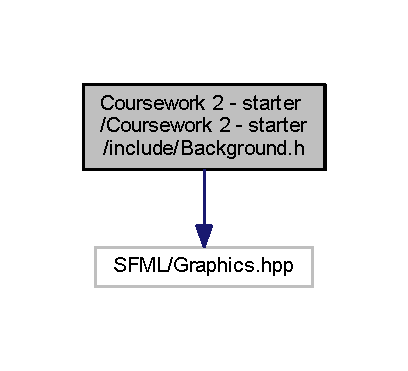
\includegraphics[width=196pt]{_background_8h__incl}
\end{center}
\end{figure}
This graph shows which files directly or indirectly include this file\+:\nopagebreak
\begin{figure}[H]
\begin{center}
\leavevmode
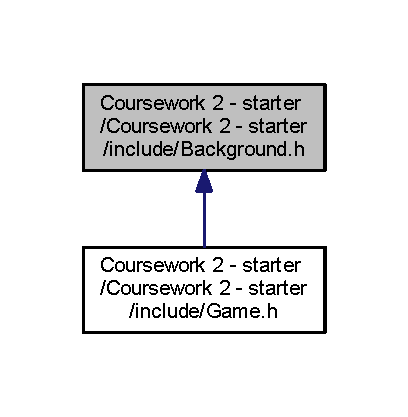
\includegraphics[width=196pt]{_background_8h__dep__incl}
\end{center}
\end{figure}


\subsection{Detailed Description}
This class builds a fixed background, and because of that it doesnt really pass many arguments or have any special reuseability to it, its kind of just a seperate class that builds once instance of a background.

If I did not struggle with some things I would spend time passing these backgrounds in thorugh file. 